\documentclass[aspectratio=169]{beamer}

\usepackage{fontspec}
\usepackage[croatian]{babel}
\usepackage{polyglossia}
\setmainlanguage{croatian}
\setmainfont{Times New Roman}

\usepackage{graphicx}
\usepackage{hyperref}
\usepackage{listings}
\usepackage{xcolor}

\usetheme{Madrid}
\usecolortheme{default}

\setbeamertemplate{navigation symbols}{}
\setbeamertemplate{footline}[frame number]

\title{ZORA}
\subtitle{Platforma za organizaciju rada}
\author{Tomislav Nebes}
\date{Ožujak 2025}

\begin{document}

\begin{frame}
    \titlepage
\end{frame}

\begin{frame}
    \frametitle{Sadržaj}
    \tableofcontents
\end{frame}

\section{Uvod}

\begin{frame}
    \frametitle{O aplikaciji}
    \begin{itemize}
        \item Web aplikacija za organizaciju rada
        \item Razvijena u Angular i .NET 9
        \item Moderno sučelje i jednostavna uporaba
    \end{itemize}
\end{frame}

\section{Arhitektura}

\begin{frame}
    \frametitle{Arhitektura sustava}
    \begin{center}
        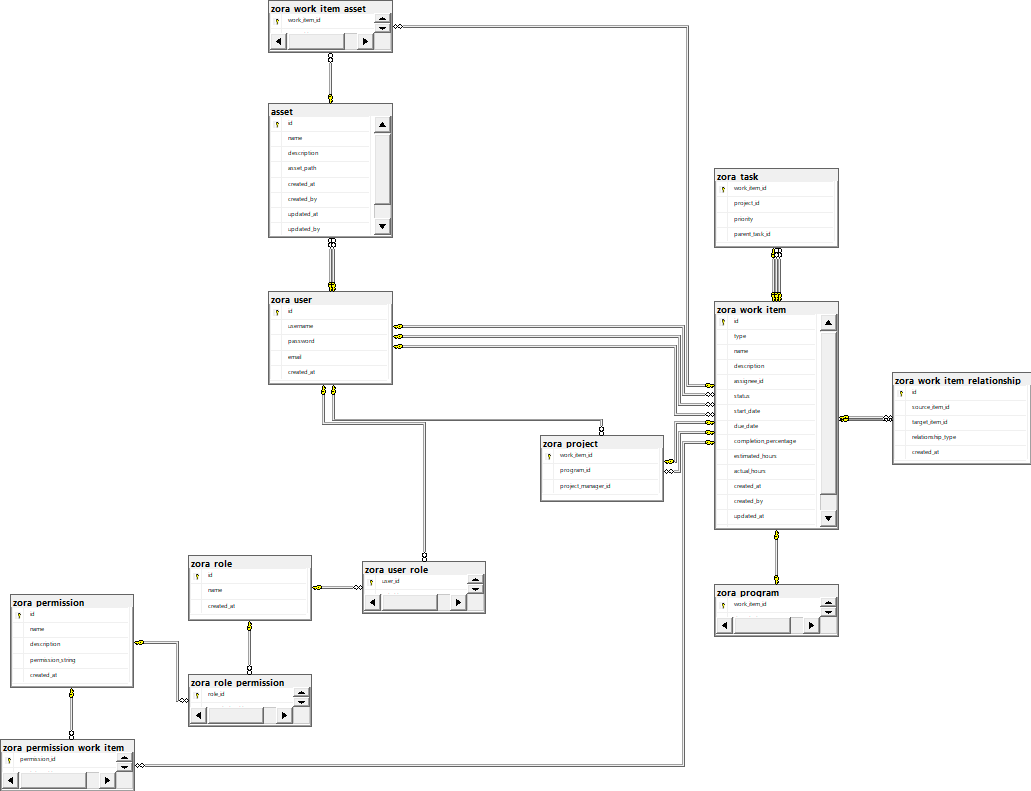
\includegraphics[height=0.8\textheight]{../zora_diagram.png}
    \end{center}
\end{frame}

\begin{frame}
    \frametitle{Deployment arhitektura}
    \begin{itemize}
        \item VPS na Ubuntu Server 22.04 LTS
        \item Nginx kao reverse proxy
        \item Let's Encrypt SSL certifikati
        \item Systemd service za backend
    \end{itemize}
\end{frame}

\begin{frame}
    \frametitle{Deployment proces}
    \begin{itemize}
        \item CI/CD kroz Jenkins
        \item Automatsko testiranje
        \item Monitoring kroz journalctl
    \end{itemize}
\end{frame}

\section{Backend}

\begin{frame}
    \frametitle{Backend tehnologije}
    \begin{itemize}
        \item .NET 9 Web API
        \item Entity Framework Core
        \item SQL Server
        \item JWT autentifikacija
        \item Swagger dokumentacija
    \end{itemize}
\end{frame}

\begin{frame}
    \frametitle{Backend struktura}
    \begin{itemize}
        \item Clean Architecture
        \begin{itemize}
            \item Controllers
            \item Services
            \item Repositories
            \item Models
            \item DTOs
        \end{itemize}
        \item Dependency Injection
        \item Middleware
        \item Custom Authentication
    \end{itemize}
\end{frame}

\begin{frame}
    \frametitle{Backend servisi}
    \begin{itemize}
        \item Systemd service konfiguracija
        \item Environment varijable
        \item Logging kroz journalctl
        \item Health checks
        \item Rate limiting
    \end{itemize}
\end{frame}

\section{Frontend}

\begin{frame}
    \frametitle{Frontend tehnologije}
    \begin{itemize}
        \item Angular 17
        \item Angular Material
        \item RxJS
        \item NgRx za state management
        \item Jest za testiranje
    \end{itemize}
\end{frame}

\begin{frame}
    \frametitle{Frontend struktura}
    \begin{itemize}
        \item Feature-based organizacija
        \begin{itemize}
            \item Core modul
            \item Shared modul
            \item Feature moduli
            \item Auth modul
        \end{itemize}
        \item Lazy loading
        \item Interceptors
        \item Guards
    \end{itemize}
\end{frame}

\begin{frame}
    \frametitle{Frontend deployment}
    \begin{itemize}
        \item PM2 process manager
        \item Nginx konfiguracija
        \item SSL/TLS
        \item Caching strategija
        \item Error tracking
    \end{itemize}
\end{frame}

\section{Demo}

\begin{frame}
    \frametitle{Demo koraci}
    \begin{itemize}
        \item Prijava u sustav
        \item Pregled glavnog zaslona
        \item Upravljanje projektima
        \item Upravljanje zadacima
    \end{itemize}
\end{frame}

\section{Demo}

\begin{frame}
    \frametitle{Demo}
    \begin{center}
        {\Huge Demo}
    \end{center}
\end{frame}

\section{Zaključak}

\begin{frame}
    \frametitle{Zaključak}
    \begin{itemize}
        \item Uspješno implementirana web aplikacija
        \item Moderne tehnologije i best practices
        \item Skalabilno i održivo rješenje
    \end{itemize}
\end{frame}

\begin{frame}
    \frametitle{Pitanja?}
    \begin{center}
        \Huge Hvala.
    \end{center}
\end{frame}

\end{document} 